This chapter describes the methods and materials used throughout the study to address the research questions of the study (Section \todo{add section number}).
Details of the modelling set-up, including initial and boundary conditions are included in this chapter.

\section{Air Quality Modelling} \label{s:modelling}

Photochemical models are used to predict future air quality scenarios.
A large array of these models are used depending on the study focus, for example, global photochemical models can predict air quality on a global scale and include the relevant chemical and dynamical processes whereas an urban model focuses on a particular urban area and includes the relevant processes (such as topography, local emission source) to the area being studie.
Despite differing scopes between models, there are a number of common inputs including emissions of chemical species into the model, transport of the species, atmospheric physical and chemical transformation and numerical solutions to the applicable differential equations.

Models are usually defined as either Eulerian or Lagrangian, with Eulerian models constituting most of the models used in the air quality modelling community \citep{Russell:2000}.
Eulerian models describe the atmosphere by fixed computational cells where species enter in and out of the cell walls and the concentrations of the species within each cell are calculated as a function of time. 
Whilst Lagrangian models simulate changes of selected air parcels during advection through the atmosphere, hence there is no mass exchange between the surroundings and the air parcel (besides the emissions) and the model calculates concentrations at different locations at different times \citep{Seinfeld:2006}. 

Photochemical models also have different dimensions, ranging from zero-dimensional (box model) to three-dimensional models where the simplicity and computing power increase with the dimension of the model.
3-D models calculate atmospheric concentrations as a function of latitude, longitude, altitude and time. 
While 2-D models assume that concentration is a function of latitude and altitude (but not longitude) and time.
Column models (or 1-D models) use concentrations that are a function of time and height.
Box models are the simplest type of a model and have uniform atmospheric concentrations that are only a function of time \citep{Seinfeld:2006}.

Box models lack physical realism and essentially focus on processes relevant to a point in the atmosphere.
Despite the lack of realism, box models are extremely useful for studying the detailed processes that influence air quality.
Examples of modelling studies that have used box models include \citet{Bin:2007}, \citet{Li:2014b} and \citet{Noelscher:2014}.

All photochemical models numerically solve the chemical species conservation equation which describes the processes affecting the concentration of the different species:
\begin{equation} \label{e:conc}
    \begin{split}
        \frac{\partial c_i}{\partial t} \hspace{2mm} + \hspace{2mm} \nabla \cdot \bar{U}c_i \hspace{2mm} = \hspace{2mm} \nabla \rho D \nabla(c_i/\rho) \hspace{2mm} + \hspace{2mm} R_i(c_1, c_2, \dots, c_n, T, t) \\ + \hspace{2mm} S_i(\bar{x}, t), \hspace{5mm} i = 1, 2, \dots, n.
    \end{split}
\end{equation}
In Eq.~\eqref{e:conc}, $c_i$ is the concentration (in mass or volume) of species $i$, $\bar{U}$ is the wind velocity vector, $D_i$ is the molecular diffusivity of species $i$, $R_i$ is the rate of concentration change of species $i$ through chemical reactions, $S_i(\bar{x}, t)$ is the source or sink of $i$ at location $\bar{x}$, $\rho$ is the air density and $n$ is the number of predicted species.
$R$ may also be a function of meteorological parameters such as temperature $T$ and $S$ includes emission and deposition processes affecting $i$ \citep{Russell:2000}.
\todo{re-word this as too similar to citation}

The dimension and type of the model determine the set of differential equations that will be solved at each time step of the model run. 
Numerical methods to determine the concentration of species $i$ in Eq.~\eqref{e:conc} vary between models, examples include Runge-Kutta \citep{Sandu:1997b}, Finite Element \citep{Russell:2000} or Rosenbrock methods \citep{Sandu:1997a}.

Initial and boundary conditions are required to numerically solve the system of differential equations.
Boundary conditions are typically the most difficult input to set accurately as this requires knowledge of the investigated species concentrations and transport at the boundary edges (if applicable) of the model grid.  
Setting the initial conditions involves fixing the starting concentrations of the species being studied, these conditions are dependent on the area being studied and whether it is an urban or rural area, amongst other considerations. 

\subsection{Model Description and Setup} \label{ss:model_setup}
In order to assess the detailed processes producing tropospheric ozone within general air quality modelling, we used a box model to focus on the gas-phase chemistry affecting tropospheric ozone.
All simulations in this study were performed using the MECCA (Module Efficiently Calculating the Chemistry of the Atmosphere) box model developed by \citet{Sander:2005} that was adapted to include MCM~v3.1 chemistry as described in \citet{Butler:2011}.
The MECCA box model has been used for numerous detailed process studies of atmospheric gas-phase chemistry including \citet{Kubistin:2010}, \citet{Xie:2008} and \citet{Lourens:2016}.

MECCA is written using the FORTRAN programming language and runs on UNIX/Linux platforms.
The setup of MECCA that we used uses the KPP (Kinetic Pre-Processor) \citep{Damian:2002} to efficiently setup up the system of differential equations (Eq.~\eqref{e:conc}).
KPP processes the specified chemistry scheme in the chemical mechanism and generates Fortran code that is then compilied by MECCA.
KPP also has numerous choices for the numerical solver used to numerically determine the concentrations of all the species described by the chemistry.
We have used a Rosenbrock solver (the ros3 option) throughout the study.

Aside from the chemistry, MECCA also calculates physical parameters at every time step of the simulations.
In our simulations, the pressure, temperature, relative humidity and boundary layer height are held constant at the set values of Table~\ref{t:model_setup}.
The specific changes to these parameters that were systematically varied to answer the research question related to \todo{add section} are detailed in the relevant publication (Chapter ). \todo{TBC about this}

\begin{table}
    \begin{center}
        \caption{General settings used for MECCA box model in this study}
        \begin{tabular}{ll}
            \hline \hline
            \textbf{Model Parameter} & \textbf{Setting} \\
            \hline \hline
            Pressure & $1013$ hPa \\
            Temperature & $293$ K \\
            Relative Humidity & $81$ \% \\
            Boundary Layer Height & $1000$ m \\
            Latitude & $34\degree$ N \\
            Starting Date and Time & 27th March 06:00 \\
            Model Time Step & $20$ mins \\
            Model Run Time & $7$ days \\
            \hline \hline
        \end{tabular}
        \label{t:model_setup}
    \end{center}
\end{table}

Photolysis rates in this study are calculated by using a paramaterisation that calculates the photolysis rate as a function of the solar zenith angle.
This paramaterisation requires the degree of latitude for the study to be a defined variable in MECCA, we have chosen the $34\degree$ N latitude which is roughly that of the city of Los Angeles.
The simulations start at the spring equinox (27th March) at 6am and allowed to run for seven diurnal cycles.

In our setup of MECCA, all fluxes into and out of the box are handled by KPP.
The chemical mechanism file, processed by KPP, includes specific pseudo-unimolecular reactions specifying the emissions and dry deposition of chemical species along with the relevant rate.
The chemical species that are emitted into the model and the emission rates are read into the model using a namelist file.
Namelist files are also used to specify the initial conditions of chemical species and the mixing ratios of those chemical species that are fixed throughout the model.
In all simulations, methane (\ce{CH4}) was fixed to 1.75 ppmv while carbon monoxide (CO) and \ce{O3} are initialised at 200 ppbv and 40 ppbv and then allowed to evolve freely.

\section{Chemical Mechanisms} \label{s:chemical_mechanisms}
The atmospheric chemistry in AQ models is described by the chemical mechanism used by the AQ model. 
The chemical mechanism includes rate coefficients, reaction pathways with the corresponding branching ratios, photolysis rates and reaction products which are required to solve the concentrations of each chemical species within the system using Equation \eqref{e:conc}.

Different modelling scopes and models determine the level of chemical detail of the chemical mechanism used by the AQ model, thus many different chemical mechanisms have been developed by the AQ modelling community.
The level of detail included in the chemical mechanism determines the amount of computing resources required for the model simulations, hence the chemical mechanism in a 3-D model will typically be less detailed than the chemical mechanism used by a box model.

Chemical mechanisms range from highly-detailed (explicit) chemical mechanisms to the less-detailed lumped-structure and lumped-molecule chemical mechanisms.
The self-generating chemical mechanism of \citet{Aumont:2005} is an example of an explicit chemical mechanism and includes many thousands of reactions outlining the degradation chemistry of VOCs, outlining even the reactions generating degradation products of minor importance in the atmosphere.
Near-explicit chemical mechanisms, such as the Master Chemical Mechanism (MCM) of \citet{Jenkin:1997}, \citet{Jenkin:2003}, \citet{Saunders:2003}, are less-detailed than self-generating mechanisms but still contain many thousands of reactions and as such are mainly used in box models.
The MCM representation of VOC degradation chemistry is discussed in more detail in Sect.~\ref{ss:near_explicit}.

Many other chemical mechanisms have been developed to describe atmospheric chemistry using less-detailed descriptions as those used by explicit and near-explicit chemical mechanisms so that these chemical mechanisms are computationally efficient for use within 3-D models.
These reduced chemical mechanisms have been developed using a number of different techniques which ultimiately lead to aggregating (lumping) VOC into mechanism species, these mechanism species are then degraded in such a way that the chemical production of ozone is similar to that from observational records.
The first part of this study compares the maximal ozone produced from a number of reduced chemical mechanisms, listed in Table~\ref{t:mechanisms}, a description of the different reduction techniques used by the reduced mechanisms is found in Sect.~\ref{ss:lumped_intermediate}, Sect.~\ref{ss:lumped_molecule} and Sect.~\ref{ss:lumped_structure}.
The main results from the chemical mechanism comparison study are presented in Sect.~\ref{s:chemical_mechanism_results}.

\begin{table}
    \begin{center}
        \caption{Chemical mechanisms used in the study.}
        \scalebox{.85}[.85]{\begin{tabular}{lll}
                \hline \hline
                \textbf{Chemical Mechanism} & \textbf{Lumping Type} & \textbf{Reference} \\
                \hline \hline
                \multirow{3}{*}{MCM v3.1 and v3.2} & \multirow{3}{*}{No lumping} & \citet{Jenkin:1997}, \citet{Jenkin:2003} \\
                & & \citet{Saunders:2003}, \citet{Bloss:2005} \\
                & & \citet{MCM_Site} \\
                CRIv2 & Lumped intermediates & \citet{Jenkin:2008} \\
                MOZART-4 & Lumped molecule & \citet{Emmons:2010} \\
                RADM2 & Lumped molecule & \citet{Stockwell:1990} \\
                RACM & Lumped molecule & \citet{Stockwell:1997} \\
                RACM2 & Lumped molecule & \citet{Goliff:2013} \\
                CBM-IV & Lumped structure & \citet{Gery:1989} \\
                CB05 & Lumped structure & \citet{Yarwood:2005} \\
                \hline \hline
            \end{tabular}
        }
        \label{t:mechanisms}
    \end{center}
\end{table}

\subsection{Near-Explicit Chemical Mechanisms} \label{ss:near_explicit}
The Master Chemical Mechanism (MCM~v3) is a near-explicit mechanism describing the chemical degradation of 107 non-aromatic VOCs in \citep{Saunders:2003} and 18 aromatic VOCs in \citep{Jenkin:2003}. 
The MCM~v3.2 was used as the reference mechanism for this study as it was the most recent version of the MCM at the time of the first experiments related to the chemical mechanism study; the MCM~v3.2 was obtained from the world wide web (\mbox{\url{http://mcm.leeds.ac.uk/MCMv3.2/}}).
In total, the MCM~v3.2 has $12,691$ reactions including $4351$ organic compounds and $46$ inorganic compounds. 
The primary VOCs represented by the MCM~v3.2 were determined by which VOC have the most emissions (by mass) as listed by the UK National Atmospheric Emissions Inventory and makes up about 70\% of the mass emissions of unique species achieved.

Each primary VOC and each degradation product, is individually degraded until it is broken down to \ce{CO2}, \ce{H2O}, CO or an organic product (or radical) already represented by the MCM \citep{Jenkin:1997}. 
\citet{Jenkin:1997} outlines the main assumptions used when developing the MCM in order to reduce the number of chemical species and reactions, these include:
\begin{enumerate}
    \item limiting the number of product channels resulting from reaction with the OH radical by disregarding pathways of low probability,
    \item representing permutation (self and cross) reactions of organic peroxy radicals by a single parameterised reaction, and
    \item simplifying the degradation chemistry, especially for those products deemed to be of minor importance.
\end{enumerate}

\begin{figure}
    \begin{center}
        \caption[Flowchart of VOC degradation represented by the MCM]{Flowchart of the major reactions of primary VOCs, intermediates and products considered in the MCM. Taken from Fig.~1 in \citet{Saunders:2003}}
        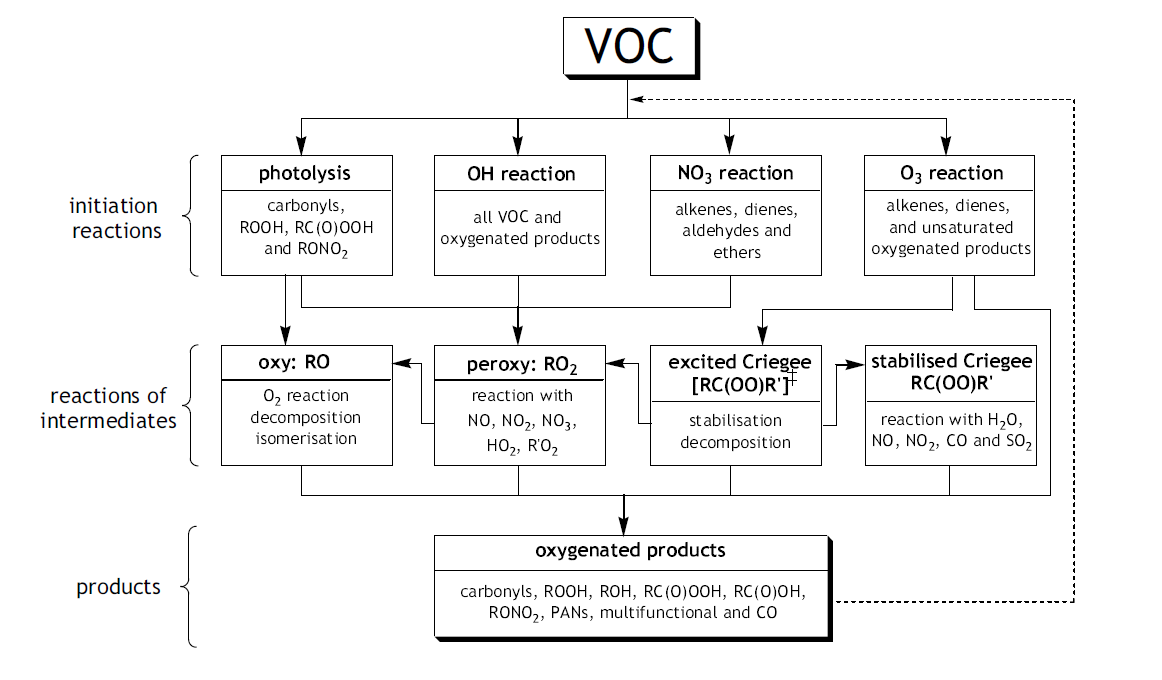
\includegraphics[width=\textwidth]{MCM_scheme.png}
        \label{f:MCM_scheme}
    \end{center}
\end{figure} 

Figure \ref{f:MCM_scheme} shows the reaction pathways represented in the MCM of the primary VOC.
The main reaction pathway for VOC degradation is by reaction with the OH radical, while ozonolysis is only important for alkenes, dienes, monoterpenes, some aromatic VOCs and some unsaturated oxygenated products. 
Reaction with the \ce{NO3} radical is mainly important during the night-time and only included for alkenes, dienes, aromatics, aldehydes and ethers.
Rate constants and branching ratios of the reactions represented in the MCM~v3.2 are those recommended by IUPAC.
If no data was available then they are estimated using structure activity representation (SAR) or group reactivity (GR) methods.

The degradation products of the primary VOCs are also treated in detail, with the first generation products also degraded further as part of the MCM. 
Those degradation products having significant tropospheric concentrations are treated in detail by the MCM otherwise the further degradation is limited to reaction with the OH radical. 
Those products deemed of minor importance are also greatly simplified whilst retaining product lifetimes and maintaining the carbon and nitrogen balance. 

\subsection{Lumped Intermediate Chemical Mechanisms} \label{ss:lumped_intermediate}
Chemical mechanisms which aggregate (lump) the degradation products rather than primary VOC are called lumped intermediate chemical mechanisms.
The Common Representative Intermediates (CRI) chemical mechanism \citep{Jenkin:2008} is an example of a lumped intermediate mechanism.

The CRI is a reduced version of the MCM that can be used in 3-D AQ models.
Reducing the complexity of the MCM was achieved by representing many degradation products (intermediates) in the CRI by a single mechanism species, rather than lumping primary VOC into a mechanism species.
These intermediates are designed to produce the same amount of ozone as when using the MCM.
The CRI~v2 was used in this study and the intermediates in this version of the CRI mirror the ozone production from the MCM~v3.1.

The CRI~v2 is available online (\mbox{\url{http://mcm.leeds.ac.uk/CRI}}) in a full version and further reduced variants that include even further reductions to the chemistry represented in MCM~v3.1 by also lumping VOCs into lumped mechanism species.
\citet{Jenkin:2008} describes the main assumptions made in order to condense the organic chemistry of the MCM~v3.1 to the lumped intermediate chemistry of the CRI~v2, while \citet{Watson:2008} describes the further reductions made to the CRI~v2 to produce the five lumped emission variants.
The most reduced version of the CRI~v2 has also been implemented into the widely used 3-D regional model WRF-CHEM as described in \citet{Archer-Nicholls:2014}.

The approach used to develop the CRI involves determining the potential number of NO-to-\ce{NO2} conversions by the peroxy radicals formed during the degradation of a VOC, this is called the CRI-index.
The CRI-index is thus the potential number of ozone molecules produced during the degradation of a VOC as the number of potential NO-to-\ce{NO2} conversions by peroxy radicals is directly related to the potential number of \ce{O3} molecules (Sect. \todo{add section}).
A single ``common representative'' is created to represent a part of the secondary degradation of a large number of species based on the CRI-index that was calculated based on the description of the degradation of the VOC in the MCM \citep{Jenkin:2008}.
This approach greatly reducing the number of species and reactions in the CRI compared to the near-explicit representation of the MCM.

The mechanism intermediate species are further optimised by performing multi-day model runs comparing the ozone produced from a single VOC in the CRI~v2 to that in MCM~v3.1.
These model runs were performed for each of the primary VOC represented in the MCM~v3.1 and CRI~v2, starting with the smallest VOC of a particular functional group and only moving to the next largest VOC once the ozone production was optimised to that of the MCM~v3.1.
The primary criterion in these tests was ozone formation, the ozone formation of the mechanism intermediate species was optimised to that in the MCM~v3.1 using a non-linear least squares fitting and the agreement was improved by varying the OH-reactivity and photolysis rate of the intermediate species.
The individual testing of the intermediates for each VOC also showed that some intermediates did not directly follow the CRI-index rule and in-place adjustments were required to retain the ozone formation in the MCM~v3.1.
This appraoch was used for OH, \ce{O3} and \ce{NO3} initiated degradation \citep{Jenkin:2008}.

Despite the large reductions to the MCM~v3.1 chemistry to produce the CRI~v2 described in \citet{Jenkin:2008}, the number of reactions are still too many to guarantee computational efficiency for use in 3-D models.
Further reductions were made by lumping VOC emissions to produce five further reduced variants of the CRI~v2; the methodology for these reductions is described in \citet{Watson:2008} and summarised below.

The focus of the reductions to the full CRI~v2 was on reducing the number of species and reactions representing anthropogenically emitted VOC, as on a global scale these VOC are less significant than biogenically emitted VOC.
The primary VOC represented by the full CRI~v2 were reduced into lumped species based upon two methods, first by re-distributing VOCs of minor importance into lumped mechanism species that represent the chemistry of separate functional classes (alkane, alkene, aromatic, alcohol/ether, aldehyde, ketone, ester/acid).
POCPs of the primary VOC being lumped into mechanism species were used to determine the ozone production from the primary VOC and then select the appropriate mechanism species.
This approach created three reduced variants (CRI~v2-R1, CRI~v2-R2 and CRI~v2-R3), with progressively increased lumping of the primary VOC \citep{Watson:2008}.

The second approach to reducing the CRI~v2 chemistry involved stricter reductions by using definitions of individual VOC emissions from the Global Emissions Inventory Activity (GEIA).
Again, POCP values of the individual VOC were used to assign the lumped mechanism species.
This approach produced the two most reduced variants of the CRI~v2--CRI~v2-R4 and CRI~v2-R5, where the latter is the most reduced form of the CRI~v2 \citep{Watson:2008}.
A summary of the five reduced variants of the CRI~v2 compared to the full CRI~v2 is presented in Table~\ref{t:CRI_summary}.

\begin{table*}
    \centering
    \caption[Summary of the CRI~v2 and its five reduced variants.]{Summary of the CRI~v2 and its five reduced variants. Data from Table~1 in \citet{Watson:2008}.}
    \label{t:CRI_summary}
    \begin{threeparttable}
        \centering
        \scalebox{0.88}[0.88]{\begin{tabular}{lllllll}
                \hline \hline
                \textbf{CRI version} & \textbf{v2} & \textbf{v2-R1} & \textbf{v2-R2} & \textbf{v2-R3} & \textbf{v2-R4} & \textbf{v2-R5} \\
                \hline \hline
                Primary VOCs & $115$ & $67$ & $55$ & $42$ & $33$ & $22$ \\
                Species \tnote{a} & $434 (4361)$ & $373 (3466)$ & $352 (3099)$ & $296 (2649)$ & $219 (1983)$ & $195 (1244)$ \\
                Reactions \tnote{a} & $1183 (12775)$ & $1012 (10150)$ & $988 (9099)$ & $882 (7833)$ & $643 (5884)$ & $555 (3670)$ \\
                \hline \hline
            \end{tabular}
        }
        \begin{tablenotes}
            \item[a] Data in brackets represents the number of species and reactions required to\\degrade the same VOCs in the MCM~v3.1.
        \end{tablenotes}
    \end{threeparttable}
\end{table*}

\subsection{Lumped Molecule Chemical Mechanisms} \label{ss:lumped_molecule}
Lumped molecule chemical mechanisms reduce atmospheric chemistry by aggregating primary VOC into mechanism species; this is the most common technique used when developing a reduced chemical mechanism.
Different chemical mechanisms use different approaches when creating these mechanism species that are used represent a multitude of primary VOC.
Typically NMVOC, such as isoprene, ethane and ethene, that make up a large fraction of NMVOC emissions are represented by dedicated (explicit) species and mechanism species are used to represent specific groups of NMVOC.
These lumped mechanism species typically represent NMVOC based on functional group or OH-reactivity.
Table~\ref{t:mechanisms} lists the lumped-molecule chemical mechanisms used in this study and Table~\ref{t:lumped_molecule} provides further information about these chemical mechanisms.
\begin{table}
    \centering
    \caption{Explicitness of each of the lumped-molecule chemical mechanisms listed in Table~\ref{t:mechanisms}}
    \label{t:lumped_molecule}
    \begin{tabular}{llll}
        \hline \hline
        \textbf{Chemical} & \textbf{Number of} & \textbf{Number of} & \textbf{Number of} \\
        \textbf{Mechanism} & \textbf{Primary VOC} & \textbf{Species} & \textbf{Reactions} \\
        \hline \hline
        MOZART-4 & $20$ & $85$ & $157$ \\
        RADM2 & $21$ & $63$ & $157$ \\
        RACM & $25$ & $77$ & $237$ \\
        RACM2 & $40$ & $120$ & $363$ \\
        \hline \hline
    \end{tabular}
\end{table}

\subsubsection{MOZART}
The Model for OZone and Related chemical Tracers (MOZART) chemical mechanism is an example of a lumped molecule chemical mechanism used in global and regional 3-D models.
MOZART was developed for global chemical transport models and describes chemical processes within the boundary layer, free troposphere and stratosphere.
MOZART-4 \citep{Emmons:2010} is the version used in this study and includes updates to the tropospheric chemistry from the previous MOZART-2 version \citep{Horowitz:2003}; MOZART-3 \citep{Kinnison:2007} provided updated stratospheric chemistry.

MOZART-4 represents organic VOCs of methane, ethane, propane, ethene, propene, isoprene and formaldehyde by explicit species.
Lumped mechanism species, BIGALK, BIGENE and TOLUENE, are used to represent alkanes and alkenes with four or more carbon atoms and all aromatic VOC \citep{Emmons:2010}.
Thus, the lumping species used by MOZART are based on the functionality of the VOC.
There are no mechanism species representing emissions of esters, ethers or chlorinated NMVOC, when representing emissions of these less-reactive NMVOC are added to the BIGALK mechanism species as this has the slowest OH-reactivity.

MOZART-4 is also capable of representing aerosol chemistry and directly calculating both photolysis and dry deposition rates.
For the purpose of this study, we were only interested in gas-phase chemical processes occuring with the boundary layer and so all processes relating to stratospheric, free troposphere and aerosol processes were not used.
We also used the MCM approach to calculating photolysis and dry deposition rates.

\subsubsection{RADM2}
One of the older lumped molecule, but still widely used, chemical mechanisms is the second version of the Regional Acid Deposition Model (RADM2) originally described in \citet{Stockwell:1990}.
RADM2 is typically used in regional modelling studies and the chemical mechanism has been used extensively since its inception.

The organic VOC methane, ethane, ethene, isoprene and formaldehyde are represented explicitly in RAMD2.
RADM2 uses lumped mechanism species to represent many VOC based upon the OH-reactivity and functional group of the VOC.
In particular, there are three mechanism species (HC3, HC5, HC8) representing three types of hydrocarbons based on their OH-reactivity.
These three species are then used to not only represent alkanes, but also many other species -- such as alcohols, ethers, chlorinated VOC -- based on their OH-reactivity.

All alkenes having more than two carbons are represented by either OLT or OLI depending on the position of the double bond (OLT: terminal alkenes and OLI: internal alkenes).
The exception to this is isoprene, whose degradation is treated by an explicit species, due to the importance of isoprene chemistry as it is globally the VOC with the most emissions.

Aromatic VOC are represented by TOL, XYL or CSL depending on whether their OH-reactivity is slow, fast or they are hydroxy-substituted.
Carbonyls (aldehydes and ketones) and organic acids are also represented by lumped mechanism species
Typically the NMVOC having the least number of carbons (e.g. formaldehyde and formic acid) is represented by an explicit species and then all other species from that functional group are represented by a lumped species.

The reaction rate coefficients of the lumped mechanism species were obtained by using a weighted mean of all the rate coefficients of the organic species aggregated into the model species, this was done to account for the difference in reactivities between the model and chemical species.
The secondary degradation of the lumped species is described by chemistry that takes into account all the known VOC that are represented by the lumped species.

RADM2 reduces the number of peroxy radicals that need to be represented by using an operator species (XO2) that converts NO to \ce{NO2} in an attempt to replicate the ozone produced by NMVOC when represented by the mechanism species.
Thus, XO2 is one such mechanism species that appears in the secondary degradation of most of the lumped mechanism species.
Another way of reducing the number of peroxy radicals is that only reactions of \ce{RO2} with \ce{HO2}, \ce{CH3O2} and \ce{CH3CO3} are included as these are the most abundant \ce{RO2}.

\subsubsection{RACM}
\citet{Stockwell:1997} describes the Regional Atmospheric Chemistry Mechanism (RACM) which is an updated to the RADM2 chemical mechanism.
RACM includes lumped mechanism species not included in RADM2 such as API and LIM to represent cyclic terpenes with one double bond and all other cyclic terpenes.

Once again, the primary VOC are grouped into lumped mechanism species based upon functional group similarity and OH radical reactivity. 
The final mechanism species was determined by first grouping hundreds of anthropogenic VOCs into $32$ emission categories and then finally aggregating into the final $16$ lumped mechanism species. 

The secondary chemistry of many of the lumped mechanism species included in both RADM2 and RACM was extensively updated which meant the inclusion of many new and additional mechanism species produced during the degradation of these lumped primary species.
These product species are calculated as a weighted mean of the product yields of all the chemical species represented by the model species, where the individual yields are taken from literature. 

The same approach to representing \ce{RO2}-\ce{RO2} reactions as used in RADM2 is used in RACM. 
Further details for calculating the reaction rate coefficients are described in \citet{Kirchner:1996}.

\subsubsection{RACM2}
RACM was further extended and updated to RACM2, described in \citet{Goliff:2013}, once again the main updates included more lumped mechanism species to represent primary VOC emissions as well as updates to the secondary chemistry of lumped mechanism species.
Alkane and alkene chemistry is largely unchanged from RACM except for some updates to reaction rate coefficients,
Moreover, there were no major changes to the approach used when describing gas-phase chemistry from RADM2 or RACM.

Aromatic VOC and subsequent secondary chemistry was overhauled in RACM2 from RACM.
RACM2 represents aromatic VOC by eight mechanism species instead of three species as in RACM, with explicit representation of benzene and each xylene isomer having its own mechanism species.
The secondary chemistry of the aromatic VOC was updated to be similar to that of the MCM, with differences arising from the different treatments of gas-phase chemistry in the MCM and RACM2.
The main difference is the different treatment of \ce{RO2}-\ce{RO2} reactions.

Acetone and methyl ethyl ketone (MEK) are now treated as separate species rather than being represent as a single mechanism species, KET, in RADM2 and RACM.
Alcohols are now also represented in RACM2, whereas in the previous versions, alcohols were represented by HC3, HC5 or HC8.

\subsection{Lumped Structure Chemical Mechanisms} \label{ss:lumped_structure}
The technique used by lumped-structure chemical mechanisms to reducing atmospheric chemistry is to express VOC emissions as permutations of building blocks that represent the structure of the emitted VOC.
Thus, each lumped-structure chemical mechanism includes a number of these building blocks which are then emitted according to the initial VOC emissions being studied.
The Carbon Bond mechanism is the most widely used lumped-structure chemical mechanism and in the first part of this thesis we have looked at the fourth version (CBM-IV, \citep{Gery:1989}) and the fifth version (CB05, \citep{Yarwood:2005}).
Both Carbon Bond versions include mechanism species representing the different carbon bonds present in typically emitted VOC, the representation of the carbon bonds included in CBM-IV and CB05 are outlined in Table~\ref{t:lumped_structure}.
\begin{table} 
    \centering
    \caption{Carbon bonds and mechanism species represented in CBM-IV and CB05.}
    \label{t:lumped_structure}
    \begin{tabular}{ll}
        \hline \hline
        \textbf{Mechanism Species} & \textbf{Carbon Bond} \\
        \hline \hline
        PAR & \ce{C-C} \\
        OLE & \ce{C=C} \\
        ALD2 & \ce{C=O} \\
        \hline \hline
    \end{tabular}
\end{table}

\subsubsection{CBM-IV}
The fourth version of the Carbon Bond mechanism was developed to represent the chemistry producing ozone in polluted urban conditions and is described in \citet{Gery:1989}.
CBM-IV represents $20$ organic species and requires $46$ reactions to fully represent the secondary chemistry.
Explicitly represented emitted NMVOC are those with the most significant emissions: isoprene, ethene and formaldehyde.
In addition to the mechanism species listed in Table~\ref{t:lumped_structure}, there are mechanism species representing both slower and faster reacting aromatic VOC (TOL and XYL).
Acetaldehyde (ALD2) is also represented as it is an important degradation product of the secondary chemistry from a number of VOC.
CBM-IV uses an operator species (XO2) to represent NO to \ce{NO2} conversion by organic peroxy radical, similar to many lumped-molecule chemical mechanisms.  

NMVOC emissions emitted by the mechanism species are described in \citet{Hogo:1989}.
For example, if heptane, having seven carbons each with a single bond, has emissions of $1 \times 10^9$~molecules~cm$^{-3}$~s$^{-1}$ then using the CBM-IV, these emissions would be represented by $7$~PAR and thus PAR emissions would be $7 \times 10^9$~molecules~cm$^{-3}$~s$^{-1}$.
Also, propene is represented as $1$~OLE and $1$~PAR and so emissions of $1 \times 10^9$~molecules~cm$^{-3}$~s$^{-1}$  would be emitted as $1 \times 10^9$~molecules~cm$^{-3}$~s$^{-1}$ of OLE and $1 \times 10^9$~molecules~cm$^{-3}$~s$^{-1}$ of PAR.

\subsubsection{CB05}
CBM-IV was updated to CB05, described in \citet{Yarwood:2005}, to include more species representing emitted VOC.
CB05 now includes $99$ organic reactions to represent the degradation of $37$ organic species.
Mechanism species for terpenes (TERP), ethane (ETHA), aldehydes with more than three carbons (ALDX), methanol (MEOH), ethanol (ETOH) and alkenes with both internal (IOLE) and external (OLE) double bonds were included.  

In addition to updating reaction rate constants and including more mechanism species to represent atmospheric chemistry more explicitly, the CB05 was also updated to include chemistry reflecting low-\ce{NO_x} conditions.
Thus reactions involving peroxide formation, a characteristic of low-\ce{NO_x} conditions, were included in CB05.

\section{Using the Chemical Mechanisms in MECCA}
As outlined in Sect.~\ref{ss:model_setup}, the MECCA boxmodel is based upon the KPP pre-processor and so required that all chemical mechanisms listed in Table~\ref{t:mechanisms} be written in the KPP format.
The KPP format of each chemical mechanism was either obtained from the WRF/Chem \citep{Grell:2005} \todo{update citation} model, which includes KPP files of RADM2, RACM and CBM-IV for use within the model.
For all the other chemical mechanisms, the chemistry published in the original reference were adapted to the KPP format.

Some changes were made to the original chemistry specified by each chemical mechanism.
Firstly, the inorganic chemistry of the MCM~v3.2 was used in each chemical mechanism in order to focus on differences between chemical mechanisms of their representation of the secondary degradation chemistry of emitted NMVOC.
Other changes included adopting the MCM~v3.2 approaches to photolysis and peroxy-peroxy reactions, a more detailed description of these changes are found in the supplementary material of the first paper of this thesis (Chap.~\ref{c:paper_1}). \todo{Include supplementary material}
